\documentclass[aspectratio=169]{beamer}

% Configuración básica del tema
\usepackage{lmodern} % Fuente moderna
\usepackage[utf8]{inputenc} % Soporte para caracteres UTF-8
\usepackage[spanish]{babel} % Idioma español
\usepackage{amsmath} % Matemáticas avanzadas

% Tema minimalista
\usetheme{default}

% Definir colores
\definecolor{customblue}{RGB}{45, 85, 150}

% Personalización del encabezado
\setbeamercolor{frametitle}{bg=customblue, fg=white}
\setbeamercolor{section in head/foot}{fg=customblue}

% Configuración del diseño
\setbeamertemplate{frametitle}{
    \nointerlineskip%
    \begin{beamercolorbox}[wd=\paperwidth, ht=2.5ex, dp=1.5ex]{frametitle}
        \usebeamerfont{frametitle}\hspace{1em}\insertframetitle
    \end{beamercolorbox}
    \vspace{0.5em}
    \nointerlineskip%
    \rule{\paperwidth}{0.2mm}
}

\setbeamertemplate{footline}[frame number]

% Inicio del documento
\begin{document}

% Primera diapositiva: Título
\begin{frame}
    \centering
    \vspace{1.5cm}
    \Huge \textbf{Chuletario Ejercicios Tema 1} \\
    \Large Lo que Dijkstra, Anna Karlin y Donald Knuth no quieren que sepas
    \vfill
    \normalsize \textit{Metodología de la Programación} \\
    \small \textbf{Autor: Víctor Alonso} % Modifica tu nombre si lo deseas
\end{frame}

% Ejemplo de diapositiva con contenido
\section{Orden de Complejidad}

\begin{frame}{Orden de Complejidad}
    \begin{itemize}
        \item \textbf{¿Qué es?:} Estudiar el \textbf{comportamiento} de un algoritmo.
        \item \textbf{Pasos:}
        \begin{enumerate}
            \item Identificar \textbf{condición de salida} del bucle.
            \item Estimar el número de iteraciones con \textit{tablita} o fórmula.
            
            \item Plantear T(n).
        \end{enumerate}
        \item \textbf{Bro tips:} 
       \begin{itemize}
            \item Un número \textit{fijo} de iteraciones no tiene impacto en el orden.
            \item Nos da igual \textit{n} iteraciones que \textit{n-m} iteraciones.
            \[
                \forall m \in \mathbb{Z}
            \]
        \end{itemize}
    \end{itemize}
\end{frame}

\begin{frame}{Orden de Complejidad (notación matemática)}
    \begin{itemize}
        \item \textbf{T(n)}: Función de complejidad. Planteamos el problema con operaciones definidas (a, b, c...), y sumatorios para los bucles.
        \[
            T(n) = a + \sum_{i=0}^n b
        \]
        \item \textbf{Orden de complejidad equivalente:} Usamos la \textit{virgulilla} encima del \textit{igual} para decir que las expresiones son \textbf{equivalentes en cuanto a orden de complejidad}.
        \[
        T(n) = a + \sum_{i=0}^n b \overset{\sim}{=} a + bn
        \]
        \item \textbf{Polinomios}: Nos quedamos con el término \textbf{n} elevado al mayor exponente. Y ese será el O(n).
        \[
            T(n) = a + \sum_{i=0}^n b \overset{\sim}{=} a + bn
            \]
            \[
            T(n) \in \mathcal{O}(n), \ \Omega(n) \ \Rightarrow \ T(n) \in \Theta(n)
        \]
    \end{itemize}
\end{frame}

\begin{frame}{Orden de Complejidad (Bro tips)}
\textbf{¿Por qué descartamos todo lo que no sea \textit{n elevado al mayor exponente}?}
    \begin{itemize}
        \item Las funciones \textbf{se comportan igual} independientemente de los \textit{términos sueltos}.
        \item Solo nos interesa saber cómo crece. No buscamos rapidez en \textit{términos absolutos}, sino \textit{comportamientos} \textbf{eficientes}.
    \end{itemize}

    % Insertar la imagen
\begin{figure}[h!]
    \centering
    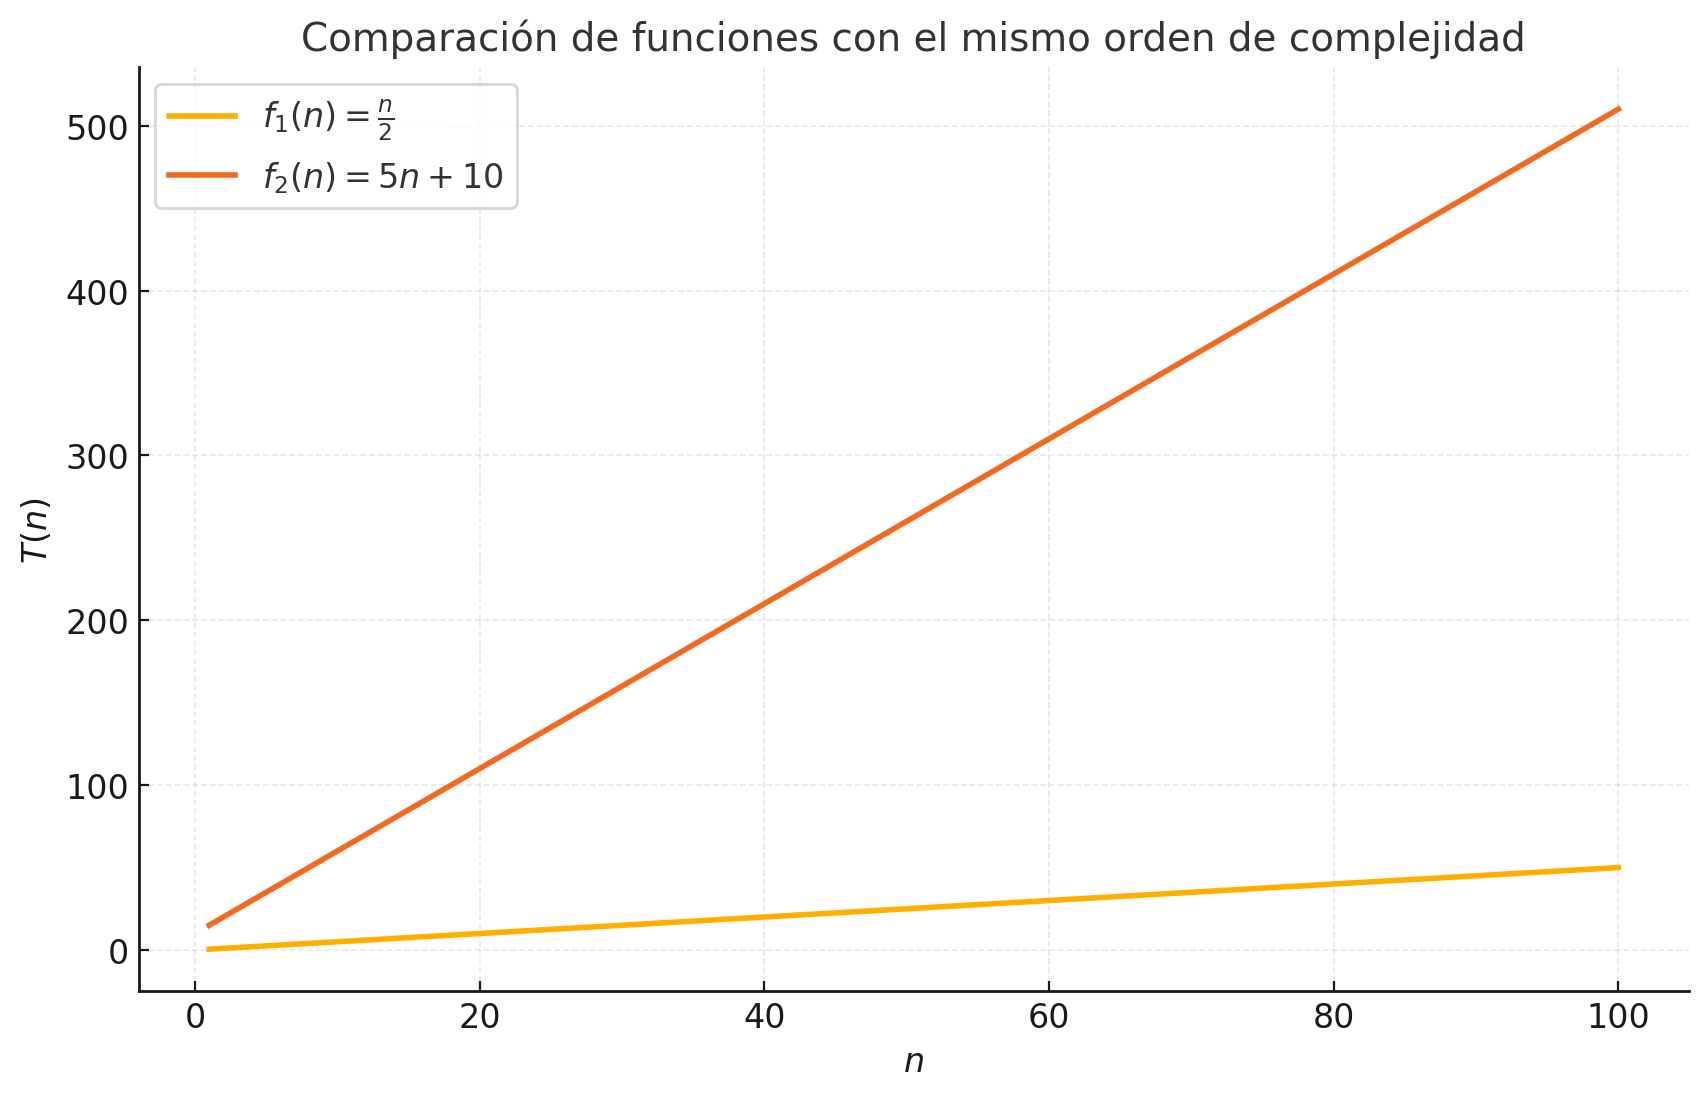
\includegraphics[width=0.5\textwidth]{orden-n.png}
    \caption{Gráfica que muestra que \(f_1(n)\) y \(f_2(n)\) tienen el mismo orden de complejidad.}
    \label{fig:orden-n}
\end{figure}
\end{frame}

\begin{frame}{Orden de Complejidad (Bro tips 2)}
\textbf{¿Por qué tienen el mismo orden de complejidad las funciones de la gráfica?}
\begin{itemize}
    \item La derivada de \(f_1(n) = \frac{n}{2}\) es \(f_1'(n) = \frac{1}{2}\), y la derivada de \(f_2(n) = 5n + 10\) es \(f_2'(n) = 5\). Ambas son constantes, lo que indica \textbf{crecimiento lineal}.
    \item Aunque \(f_2(n)\) crece más rápido que \(f_1(n)\), ambas funciones tienen el mismo tipo de crecimiento: \textbf{proporcional a \(n\)}.
    \item En términos de complejidad, \textbf{solo importa el comportamiento asintótico} para \(n\) grande, por lo que las constantes y términos independientes son irrelevantes.
    \item Esto demuestra que ambas funciones están en el mismo orden de complejidad, \(\mathcal{O}(n)\). Aunque los algoritmos \textbf{no tarden el mismo tiempo exacto}.
    \item El crecimiento de estas funciones es continuo y uniforme, a diferencia de otros tipos de crecimiento (e.g., \(n^2\) o \(\log n\)).
\end{itemize}

\end{frame}

% Nueva sección (puedes copiar y pegar este formato para añadir más diapositivas)
\section{Análisis de un bucle}

\begin{frame}[fragile]{Número de iteraciones}
\begin{verbatim}
j = n
k = 1
while j >= 1
    k = k + 1
    j = n / k
\end{verbatim}

\begin{itemize}
    \item \textbf{Buscamos condición de salida:} El bucle termina cuando \(j < 1\). Pero podemos \textit{aproximarlo} a \(j = 1\).
    \item \textbf{¿Cuándo se cumple?:} Analizamos las operaciones en \(j\):
    \begin{itemize}
        \item \(j = n / k\), por lo que \(j = 1\) cuando \(n / k = 1\), es decir, cuando \(k = n\).
        \item Como \(k\) aumenta de uno en uno (\(k = k + 1\) en cada iteración), el bucle ejecutará \(n\) iteraciones.
    \end{itemize}
    \item \textbf{Bro Tip}: A veces no hace falta \textit{tablita mágica}.
\end{itemize}
\end{frame}


\begin{frame}{Cosas que quedan bien}
\textbf{Índices del sumatorio}

\begin{itemize}
    \item Es importante fijarse en \textbf{dónde empieza el bucle} para definir correctamente el índice inferior del sumatorio.
    \item En el caso anterior:
    \[
    \sum_{k=1}^n
    \]
    El bucle empieza en \(k = 1\) y termina en \(k = n\).

    \item Sin embargo, en otros casos, el bucle puede \textit{ir al revés}. Por ejemplo el ejercicio 4. Si lo expresamos en términos de un sumatorio:
    \[
    \sum_{i=\log_5 n}^1
    \]

    \item \textbf{Bro tip:} Da igual cómo se pongan los límites del sumatorio porque representan las mismas iteraciones. Lo importante es reflejar correctamente el comportamiento del bucle.
\end{itemize}

\end{frame}

\section{Bucle anidado}

\begin{frame}{Bucle anidado y sumatorios}
\[
T(n) = a + \sum_{i=0}^n \left( b + \sum_{k=0}^n c \right)
\]

\begin{itemize}
    \item El primer sumatorio (\(\sum_{i=0}^n\)) representa el bucle exterior, el segundo sumatorio (\(\sum_{k=0}^n\)) representa el bucle interior.
    \item Resolvemos primero el sumatorio del bucle interior:
    \[
        T(n) = a + \sum_{i=0}^n \left( b + cn \right)
    \]
    \item Resolvemos después del otro sumatorio.
    \[
        T(n) = a + bn + cn^2
    \]
   \end{itemize}

   \[
T(n) = a + \sum_{i=0}^n \left( b + \sum_{k=0}^n c \right) \overset{\sim}{=} a + \sum_{i=0}^n \left( b + cn \right) \overset{\sim}{=} a + bn + cn^2
\]
\end{frame}


\begin{frame}{Bro Tips para resolver sumatorios}
\begin{itemize}
    \item \textbf{Poner \(a\), \(b\), \(c\)...:} Identifica claramente las constantes y dónde aparecen en el bucle.
    \item \textbf{Poner paréntesis:} Agrupa las operaciones correctamente para no perder términos en cada paso.
    \item \textbf{\(b\) son las operaciones antes del bucle:} Estas se SUMAN a las del sumatorio interior, y deben incluirse fuera del segundo sumatorio.
    \item \textbf{Resolver paso a paso:} Simplifica un sumatorio a la vez para evitar errores y asegurar que el resultado final sea correcto.
\end{itemize}
\end{frame}

\end{document}
